\documentclass[a4paper,12pt]{article}
\usepackage{amsmath,amsthm,amsfonts,amssymb,amscd,amstext,vmargin,graphics,graphicx,tabularx,multicol} 
\usepackage[francais]{babel}
\usepackage[utf8]{inputenc}  
\usepackage[T1]{fontenc} 
\usepackage{pstricks-add,tikz,tkz-tab,variations}
\usepackage[autolanguage,np]{numprint} 


\setmarginsrb{2.5cm}{0.5cm}{2cm}{2cm}{0cm}{0cm}{0cm}{0cm} %Gauche, haut, droite, haut
\newcounter{numexo}
\newcommand{\exo}[1]{\stepcounter{numexo}\noindent{\bf Exercice~\thenumexo} : \marginpar{\hfill /#1}}
\reversemarginpar


\newcounter{enumtabi}
\newcounter{enumtaba}
\newcommand{\q}{\textbf{\stepcounter{enumtabi} \theenumtabi)}  }
\newcommand{\qa}{\textbf{\stepcounter{enumtaba} (\alph{enumtaba})} }
\newcommand{\initq}{\setcounter{enumtabi}{0}}
\newcommand{\initqa}{\setcounter{enumtaba}{0}}

\newcommand{\be}{\begin{enumerate}}
\newcommand{\ee}{\end{enumerate}}
\newcommand{\bi}{\begin{itemize}}
\newcommand{\ei}{\end{itemize}}
\newcommand{\bp}{\begin{pspicture*}}
\newcommand{\ep}{\end{pspicture*}}
\newcommand{\bt}{\begin{tabular}}
\newcommand{\et}{\end{tabular}}
\renewcommand{\tabularxcolumn}[1]{>{\centering}m{#1}} %(colonne m{} centrée, au lieu de p par défault) 
\newcommand{\tnl}{\tabularnewline}

\newcommand{\bmul}[1]{\begin{multicols}{#1}}
\newcommand{\emul}{\end{multicols}}

\newcommand{\trait}{\noindent \rule{\linewidth}{0.2mm}}
\newcommand{\hs}[1]{\hspace{#1}}
\newcommand{\vs}[1]{\vspace{#1}}

\newcommand{\N}{\mathbb{N}}
\newcommand{\Z}{\mathbb{Z}}
\newcommand{\R}{\mathbb{R}}
\newcommand{\C}{\mathbb{C}}
\newcommand{\Dcal}{\mathcal{D}}
\newcommand{\Ccal}{\mathcal{C}}
\newcommand{\mc}{\mathcal}

\newcommand{\vect}[1]{\overrightarrow{#1}}
\newcommand{\ds}{\displaystyle}
\newcommand{\eq}{\quad \Leftrightarrow \quad}
\newcommand{\vecti}{\vec{\imath}}
\newcommand{\vectj}{\vec{\jmath}}
\newcommand{\Oij}{(O;\vec{\imath}, \vec{\jmath})}
\newcommand{\OIJ}{(O;I,J)}


\newcommand{\reponse}[1][1]{%
\multido{}{#1}{\makebox[\linewidth]{\rule[0pt]{0pt}{20pt}\dotfill}
}}

\newcommand{\titre}[5] 
% #1: titre #2: haut gauche #3: bas gauche #4: haut droite #5: bas droite
{
\noindent #2 \hfill #4 \\
#3 \hfill #5

\vspace{-1.6cm}

\begin{center}\rule{6cm}{0.5mm}\end{center}
\vspace{0.2cm}
\begin{center}{\large{\textbf{#1}}}\end{center}
\begin{center}\rule{6cm}{0.5mm}\end{center}
}


\begin{document}
\pagestyle{empty}
\titre{Contrôle : Les limites de fonctions}{Nom :}{Prénom :}{\textbf{TCOM}}{Date:}

\vspace*{0.25cm}

\exo{4} \textit{Conjecturer une limite}
\bmul{2}
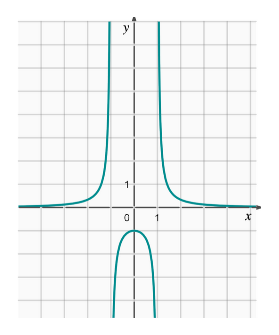
\includegraphics[scale=1.25]{limite.eps} 
\columnbreak

\vspace*{0.5cm}
Déterminer graphiquement les limites de $f$ en $-\infty$, en $+\infty$, en -1 et en 1 à gauche et à droite.\\

Indiquer les asymptotes éventuelles.
\emul



\exo{7} \textit{Calculs de limites}
\bmul{2}


\initqa \qa $\lim\limits_{\substack{x \rightarrow +\infty}} \left( x-10+e^x \right)$


\qa $\lim\limits_{\substack{x \rightarrow -\infty}} \left( x-10+e^x\right) $



\columnbreak




\qa $\lim\limits_{\substack{x \rightarrow 3 \\ x>3}} \left( \dfrac{2x-1}{3-x} \right)$


\qa  $\lim\limits_{\substack{x \rightarrow 0 \\ x>0}}\left( \dfrac{3x^3-7}{1-e^x}\right) $



\emul

\qa  $\lim\limits_{\substack{x \rightarrow +\infty }} \left( \dfrac{1}{2x\sqrt{x}}-5\right) $\\




\exo{3.5} Soit $f$ la fonction définie sur $\R \backslash \left\lbrace -2 \right\rbrace$ dont le tableau de variation est le suivant :\\

\begin{variations}
x          & \mI &       &  & -2& &  & 2& & \pI \\
\filet
$\m{f}$ &  3   &   \c & \h\pI & \bb & \mI & \c & \h1 & \d &0 \\
\end{variations}

\vspace*{0.25cm}

\noindent \initqa \qa Donner toutes les limites de $f$ qui sont renseignées dans ce tableau.\\
\qa Dans un repère, $C_f$ est la courbe représentative de $f$.\\
 Déterminer les asymptotes de $C_f$.\\
\qa Montrer que l'équation $f(x)=0$ admet une unique solution sur $\R$.\\




\exo{5.5}\\


\begin{variations}
x          & \mI &      &       & -2   &     &  &  &     &   1&   &    & \pI \\
\filet
$\m{f   }$ &  2  &   \c & \h\pI & \bb & \mI &  & \c &  \h\pI & \bb & \mI & \c & \h1 \\
\end{variations}



\noindent \initq \q Justifier que $f$ est continue sur $\R$.\\
\q Déterminer le nombre de solutions de $f(x)=0$ sur  $\R$.\\
\q \textbf{BONUS :} Déterminer la valeur des solutions $\alpha_1$ et $\alpha_2$. En déduire le signe de $f(x)$ en fonction des valeurs de $x$.\\



\end{document}
